\documentclass[../main.tex]{subfiles}

\begin{document}
\setcounter{chapter}{29}
\chapter{Déterminant}
\tableofcontents
\clearpage

\setsection{3}
\section{Exemple}
\begin{tcolorbox}[title=Exemple 30.4, title filled=false, colframe=darkgreen, colback=darkgreen!10!white]
    On considrèe l'application : 
    \begin{align*}
        \delta:\mathbb{K}^2 \times \mathbb{K}^2\to \mathbb{K}; ((a, b), (c, d)) \mapsto ad - bc
    \end{align*}
    Montrer que cette application est bien $2$-linéaire. 
\end{tcolorbox}

\begin{align*}
    \delta \left( \begin{pmatrix}
        a \\ b
    \end{pmatrix}, \begin{pmatrix}
        c \\ d
    \end{pmatrix} + \lambda \begin{pmatrix}
        c' \\ d'
    \end{pmatrix} \right) &= \delta \left( \begin{pmatrix}
        a \\ b
    \end{pmatrix}, \begin{pmatrix}
        c + \lambda c' \\ d + \lambda d'
    \end{pmatrix} \right) \\
    &= a(d + \lambda d') - b(c + \lambda c') \\
    &= ad - bc + \lambda(ad' - bc') \\
    &= \delta \left( \begin{pmatrix}
        a \\ b
    \end{pmatrix}, \begin{pmatrix}
        c \\ d
    \end{pmatrix} \right) + \lambda \delta \left( \begin{pmatrix}
        a \\ b
    \end{pmatrix}, \begin{pmatrix}
        c' \\ d'
    \end{pmatrix} \right)
\end{align*}

\setsection{10}
\section{Détermination d'une application n-linéaire sur une base}
\begin{tcolorbox}[title=Propostion 30.11, title filled=false, colframe=lightblue, colback=lightblue!10!white]
    Soit pour tout $i\in \llbracket 1, n \rrbracket$, $(e_{i,j})_{1\leq j\leq d}$ une base de $E_i$ et pour tout $(j_1, \ldots, j_n)\in \llbracket 1, d_1 \rrbracket \times \cdots \times \llbracket 1, d_n \rrbracket$, $f_{j_1, \ldots, j_n}\in F$. \\
    Alors il existe une unique application $n$-linéaire $f:E_1\times \cdots \times E_n\to F$ telle que : 
    \begin{align*}
        \forall (j_1, \ldots, j_n)\in \llbracket 1, d_1 \rrbracket \times \cdots \times \llbracket 1, d_n \rrbracket, \varphi(e_{1,j_1}, \ldots, e_{n,j_n}) = f_{j_1, \ldots, j_n}
    \end{align*}
\end{tcolorbox}

\noindent Si $(e_{i,j})_{1\leq j\leq d}$ est une base de $E_i$ alors $((e_{1, 2}, 0, \ldots, 0, \ldots, e_{1, d}, 0, \ldots, 0), \ldots, (0, \ldots, 0, e_{n, 1}, \ldots, (0, \ldots, 0, e_{n, d})))$ est une base de $E_1\times \cdots \times E_n$. (22.16), théorème de rigidité. 

\setsection{17}
\section{Caractérisation par les transpositions}
\begin{tcolorbox}[title=Lemme 30.18, title filled=false, colframe=orange, colback=orange!10!white]
    Pour qu'une forme $f$ soit antisymétrique, il faut et il suffit que l'échange de deux variables quelconques provoque un changement de signe. 
\end{tcolorbox}

\noindent Par hypothèse, si $\tau$ est une transposition alors $\varphi(x_{\tau_1}, \ldots, x_{\tau_n}) = -\varepsilon(\tau)(x_1, \ldots, x_n)$. \\
Soit $\sigma\in S_n$. On écrit $\sigma = \tau_1\circ \cdots \circ\tau_k$ avec $\tau_i$ des transpositions. Alors : 
\begin{align*}
    \varphi(x_{\sigma_1}, \ldots, x_{\sigma_n}) &= \varphi(x_{\tau_1\circ\cdots\circ\tau_k(1)}, \ldots, x_{\tau_1\circ\cdots\circ\tau_k(n)}) \\
    &= \varepsilon(\tau_1) \varphi(x_{\tau_2\circ\cdots\circ\tau_k(1)}, \ldots, x_{\tau_2\circ\cdots\circ\tau_k(n)}) \\
    &= \varepsilon(\tau_1\circ \cdots \circ \tau_k) \varphi(x_1, \ldots, x_n) \\
    &= \varepsilon(\sigma) \varphi(x_1, \ldots, x_n)
\end{align*}

\section{Une forme alternée change de signe par transposition}
\begin{tcolorbox}[title=Lemme 30.19, title filled=false, colframe=orange, colback=orange!10!white]
    Soit $\varphi$ une forme alternée. Alors pour tout $(x_1, \ldots, x_n)\in E^n$ et tout $(i, j)\in \llbracket 1, n \rrbracket^2$ avec $i\neq j$ :
    \begin{align*}
        \varphi(x_1, \ldots, x_i, \ldots, x_j, \ldots, x_n) = -\varphi(x_1, \ldots, x_j, \ldots, x_i, \ldots, x_n)
    \end{align*}
    Cela revient à dire que pour toute transposition $\tau\in S_n$, on a :
    \begin{align*}
        \varphi(x_1, \ldots, x_n) = -\varepsilon(\tau)\varphi(x_{\tau_1}, \ldots, x_{\tau_n})
    \end{align*}
    Réciproquement, si cette condition est satisfaite et si $\mathbb{K}$ n'est pas de caractéristique $2$, alors $\varphi$ est alternée.
\end{tcolorbox}

\noindent Soit $\varphi$ alternée. \\
Soit $(x_1, \ldots, x_n)\in E^n$. \\
\begin{align*}
    0 &= \varphi(x_1, \ldots, x_i + x_j, \ldots, x_j + x_i, \ldots, x_n) \\
    &= \varphi(x_1, \ldots, x_i, \ldots, x_i, \ldots, x_n) \\
    &+ \varphi(x_1, \ldots, x_i, \ldots, x_j, \ldots, x_n) \\
    &+ \varphi(x_1, \ldots, x_j, \ldots, x_i, \ldots, x_n) \\
    &+ \varphi(x_1, \ldots, x_j, \ldots, x_i, \ldots, x_n) \\
    &= \varphi(x_1, \ldots, x_j, \ldots, x_n) + \varphi(x_1, \ldots, x_j, \ldots, x_i, \ldots, x_n) \\
\end{align*}
On suppose que $\operatorname{carac}(\mathbb{K}) \neq 2$. \\
On a :
\begin{align*}
    \varphi(x_1, \ldots, x_i, \ldots, x_i, \ldots, x_n) &= \varphi(x_1, \ldots, x_i, \ldots, x_i, \ldots, x_n) \text{ (antisymétrie)} \\
\end{align*}
Donc : 
\begin{align*}
    2\varphi(x_1, \ldots, x_i, \ldots, x_i, \ldots, x_n) &= 0
\end{align*}
Donc : 
\begin{align*}
    \varphi(x_1, \ldots, x_i, \ldots, x_i, \ldots, x_n) &= 0
\end{align*}

\setsection{20}
\section{Image d'une famille liée par une forme alternée}
\begin{tcolorbox}[title=Propostion 30.21, title filled=false, colframe=lightblue, colback=lightblue!10!white]
    Soit $(x_1, \ldots, x_n)$ une famille liée et $\varphi$ une forme alternée. Alors :
    \begin{align*}
        \varphi(x_1, \ldots, x_n) = 0
    \end{align*}
\end{tcolorbox}

\noindent Si $(x_1, \ldots, x_n)$ est liée, alors on peut écrire par exemple : 
\begin{align*}
    x_1 = \sum_{i=2}^n \lambda_i x_i
\end{align*}
Donc : 
\begin{align*}
    \varphi(x_1, \ldots, x_n) &= \varphi \left( \sum_{i=2}^{n} \lambda_i x_i, x_2, \ldots x_n \right) \\ 
    &= \sum_{i=2}^{n} \lambda_i \varphi(x_i, x_2, \ldots, x_n)
\end{align*}

\section{Forme $n$-linéaire d'un espace de dimension $n$}
\begin{tcolorbox}[title=Théorème 30.22, title filled=false, colframe=orange, colback=orange!10!white]
    Soit $E$ un espace vectoriel de dimension $n$ non nulle et $(e_1, \ldots, e_n)$ une base de $E$. 
    \begin{enumerate}
        \item Il existe une unique forme $n$-linéaire $\varphi$ sur $E$ telle que $\varphi(e_1, \ldots, e_n) = 1$.
        \item Cette forme $n$-linéaire est entièrement décrite sur les vecteurs de la base par : 
        \begin{align*}
            \begin{cases}
                \varphi(e_{i_1}, \ldots, e_{i_n}) = 0 & \text{s'il existe } j\neq k \text{ tel que } i_j = i_k \\
                \varphi(e_{\sigma(1)}, \ldots, e_{\sigma(n)}) = \varepsilon(\sigma) & \text{où } \sigma\in \mathcal{S}_n
            \end{cases}
        \end{align*}
        \item Toute autre forme $n$-linéaire alternée sur $E$ est de la forme $\lambda \varphi$, où $\lambda\in \mathbb{K}$. 
    \end{enumerate}
\end{tcolorbox}

\boxed{1, 2} \\
On utilise le théorème de rigidité des applications $n$-linéaires (30.11) en fixant l'image de chaque $(e_{i_1}, \ldots, e_{i_n})$ avec $(i_1, \ldots, i_n)\in \llbracket 1, n \rrbracket^n$. 
\begin{itemize}
    \item $\varphi(e_{i_1}, \ldots, e_{i_n}) = 0$ s'il existe $i_j - i_k$ avec $j\neq k$.
    \item $\varphi(\underbrace{e_{\sigma(1)}, \ldots, e_{\sigma(n)}}_{(i_1, \ldots, i_n) \text{ fournit alors une permutation }\sigma\in \mathcal{S}_n}) = \varepsilon(\sigma) \times \underbrace{1}_{\varphi(e_1, \ldots, e_n)}$.
\end{itemize}
Le théorème nous fournit l'existence de la forme alternée et l'unicité. \\ \\

\boxed{3} \\
Soit $\psi$ une forme $n$-linéaire alternée. On pose $\lambda = \psi(e_1, \ldots, e_n)$. 
\begin{itemize}
    \item si $\lambda = 0$, par alternance (et anitsymétrie) on a $\psi(e_{i_1}, \ldots, e_{i_n}) = 0$ pour tout $i_1, \ldots, i_n$. \\
    Par rigidité, $\psi = 0 = 0\times \varphi$. 
    \item si $\lambda\neq 0$, alors $\frac{1}{\lambda}\psi(_1, \ldots, e_n) = 1$. \\
    Par unicité (1), $\frac{1}{\lambda}\psi = \varphi$. \\
    Donc $\psi = \lambda\varphi$.
\end{itemize}

\setsection{24}
\section{Exemple}
\begin{tcolorbox}[title=Exemple 30.25, title filled=false, colframe=darkgreen, colback=darkgreen!10!white]
    On considère $E = \mathbb{R}^2$, muni de sa base canonique $e = (e_1, e_2) = ((1, 0), (0, 1))$. Soit $((a, b), (c, d))\in E^2$. Montrer que : 
    \begin{align*}
        \underset{e}{\operatorname{det}}((a, b), (c, d))= ad - bc
    \end{align*}
\end{tcolorbox}

\noindent $e = ((1, 0), (0, 1))$. \\
$((a, b), (c, d))\in (E)^2$. 
\begin{align*}
    \operatorname{det}_e((a, b), (c, d)) &= \operatorname{det}_e(ae_1 + be_2, ce_1 + de_2) \\
    &= ac\times \cancel{\operatorname{det}_e(e_1, e_1)} + ad\times \operatorname{det}_e(e_1, e_2) + bc\times \operatorname{det}_e(e_2, e_1) + bd\times \cancel{\operatorname{det}_e(e_2, e_2)} \\
    &= ad \times \operatorname{det}_e(e_1, e_2) - bc \times \operatorname{det}_e(e_1, e_2) \\
    &= (ad - bc)
\end{align*}

\section{Description du déterminant par les coordonnées}
\begin{tcolorbox}[title=Théorème 30.26, title filled=false, colframe=orange, colback=orange!10!white]
    Soit $E$ un espace vectoriel de dimension $n$ non nulle et $\mathcal{B} = (e_1, \ldots, e_n)$ une base de $E$. Soit $(x_1, \ldots, x_n)$ une famille d'éléments de $E$, dont les coordonnées sont : 
    \begin{align*}
        \forall j\in \llbracket 1, n \rrbracket, x_j = \sum_{i=1}^{n} a_{i, j} e_i \quad \text{donc} \quad \operatorname{Mat}_{\mathcal{B}}(x_j) = \begin{pmatrix}
            a_{1, j} \\
            \vdots \\
            a_{n, j}
        \end{pmatrix}
    \end{align*}
    On a alors : 
    \begin{align*}
        \underset{\mathcal{B}}{\operatorname{det}}(x_1, \ldots, x_n) = \sum_{\sigma\in \mathcal{S}_n} \varepsilon(\sigma) a_{\sigma(1), 1} \cdots a_{\sigma(n), n} = \sum_{\tau\in \mathcal{S}_n} \varepsilon(\tau) a_{1, \tau(1)} \cdots a_{n, \tau(n)}
    \end{align*}
\end{tcolorbox}

\begin{align*}
    \operatorname{det}_{\mathcal{B}}(x_1, \ldots, x_n) &= \operatorname{det}_{\mathcal{B}} \left( \sum_{i=1}^{n} a_{i_1, 1} e_{i_1}, \ldots, \sum_{i=1}^{n} a_{i_n, n} e_{i_n} \right) \\
    &= \sum_{i_1=1}^{n} \cdots \sum_{i_n=1}^{n} a_{i_1, 1} \cdots a_{i_n, n} \operatorname{det}_{\mathcal{B}}(e_{i_1}, \ldots, e_{i_n}) \text{ (multilinéarité)} \\
    &= \sum_{\{i_1, \ldots, i_n\} = \llbracket 1, n \rrbracket} a_{i_1, 1} \cdots a_{i_n, n} \operatorname{det}_{\mathcal{B}}(e_{i_1}, \ldots, e_{i_n}) \text{ (alternance)} \\
    &= \sum_{\sigma\in \mathcal{S}_n} a_{\sigma(1), 1} \cdots a_{\sigma(n), n} \underbrace{\operatorname{det}_{\mathcal{B}}(e_{\sigma(1)}, \ldots, e_{\sigma(n)})}_{= \varepsilon(\sigma)} \text{ (reformulation)} \\
    &= \sum_{\sigma\in \mathcal{S}_n} \varepsilon(\sigma) a_{1, \sigma^{-1}(1)} \cdots a_{n, \sigma^{-1}(n)} \\
    &= \sum_{\tau\in \mathcal{S}_n} \epsilon(\tau) a_{1, \tau(1)} \cdots a_{n, \tau(n)}
\end{align*}

\setsection{27}
\section{Effet d'un changement de base sur le déterminant}
\begin{tcolorbox}[title=Propostion 30.28, title filled=false, colframe=lightblue, colback=lightblue!10!white]
    Soit $\mathcal{B}$ et $\mathcal{B}'$ deux bases de $E$. Alors : 
    \begin{align*}
        \underset{\mathcal{B}}{\operatorname{det}} = \underset{\mathcal{B}}{\operatorname{det} (\mathcal{B}')} \times  \underset{\mathcal{B}'}{\operatorname{det}} 
    \end{align*}
\end{tcolorbox}

\noindent D'après le corollaire (30.27), on écrit : 
\begin{align*}
    \underset{\mathcal{B}'}{\operatorname{det}} = \lambda \underset{\mathcal{B}}{\operatorname{det}} \text{ avec } \lambda\in \mathbb{K}
\end{align*}
En particulier : 
\begin{align*}
    \operatorname{det}_{\mathcal{B}'}(\mathcal{B}) = \lambda \operatorname{det}_{\mathcal{B}}(\mathcal{B}) = \lambda
\end{align*}

\setsection{29}
\section{Caractérisation des bases par le déterminant}
\begin{tcolorbox}[title=Propostion 30.30, title filled=false, colframe=lightblue, colback=lightblue!10!white]
    Soit $E$ un espace vectoriel de dimension $n$ non nulle, muni d'une base $\mathcal{B}$. Une famille $\mathcal{F}$ de cardinal $n$ est une base si et seulement si $\operatorname{det}_\mathcal{B}(\mathcal{F})\neq 0$. 
\end{tcolorbox}

\noindent D'après (30.29), si $\mathcal{F}$ est une base alors $\operatorname{det}_\mathcal{B}(\mathcal{F})\neq 0$. \\
Si $\mathcal{F}$ n'est pas une base, alors elle est liée ($|\mathcal{F}| = n$) \\
Donc $\operatorname{det}_\mathcal{B}(\mathcal{F}) = 0$ (30.21). 

\setsection{35}
\section{Déterminant d'un produit}
\begin{tcolorbox}[title=Théorème 30.36, title filled=false, colframe=orange, colback=orange!10!white]
    Soit $A$ et $B$ dans $\mathcal{M}_n(\mathbb{K})$. Alors : 
    \begin{align*}
        \operatorname{det}(AB) = \operatorname{det}(A) \operatorname{det}(B) = \operatorname{det}(BA)
    \end{align*}
\end{tcolorbox}

\noindent Soit $A, B$ dans $\mathcal{M}_n(\mathbb{K})$. On note $A_1, \ldots, A_n$ les colonnes de $A$ et $B_1, \ldots, B_n$ les colonnes de $B$. \\
On considère l'application : 
$$\varphi: (\mathbb{K}^n)^n\to \mathbb{K};(X_1, \ldots, X_n)\mapsto \operatorname{det}_{\mathcal{B_C}}(AX_1, \ldots, AX_n)$$
$\varphi$ est une forme $n$-linéaire alternée. \\
On choisit donc $\lambda\in \mathbb{K}$ tel que $\varphi = \lambda \operatorname{det}_{\mathcal{B}_C}$
On a : 
\begin{align*}
    \varphi(\mathcal{B}_C) &= \lambda \operatorname{det}_{\mathcal{B}_C}(\mathcal{B}_C) \\
    &= \lambda \\
    &= \operatorname{det}_{\mathcal{B}_C} \left( A \begin{pmatrix}
        1 \\ 0 \\ \vdots \\ 0
    \end{pmatrix}, \ldots, A \begin{pmatrix}
        0 \\ 0 \\ \vdots \\ 1
    \end{pmatrix} \right) \\
    &= \operatorname{det}_{\mathcal{B}_C}(A_1, \ldots, A_n) \\
    &= \operatorname{det}(A)
\end{align*}
Ainsi $\varphi = \operatorname{det}(A) \operatorname{det}_{\mathcal{B}_C}$. \\
Donc : 
\begin{align*}
    \operatorname{det}(A) \operatorname{det}(B) &= \operatorname{det}(A) \operatorname{det}_{\mathcal{B}_C}(\mathcal{B}_1, \ldots, \mathcal{B}_n) \\
    &= \varphi(\mathcal{B}_1, \ldots, \mathcal{B}_n) \\
    &= \operatorname{det}_{\mathcal{B}_C}(AB_1, \ldots, AB_n) \\
    &= \operatorname{det} (AB)
\end{align*}

\setsection{39}
\section{Expression des déterminants classiques}
\begin{tcolorbox}[title=Propostion 30.40, title filled=false, colframe=lightblue, colback=lightblue!10!white]
    \begin{enumerate}
        \item On a : 
        \begin{align*}
            \begin{vmatrix}
                a & b \\
                c & d
            \end{vmatrix} = ad - bc
        \end{align*}
        \item \begin{align*}
            \begin{vmatrix}
                a & b & c \\
                d & e & f \\
                g & h & i
            \end{vmatrix} = aei + bfg + cdh - gec - hfa - idb
        \end{align*}
        Soit : diagonales descendantes moins les diagonales ascendantes. 
    \end{enumerate}
\end{tcolorbox}

\begin{enumerate}
    \setcounter{enumi}{1}
    \item $\mathcal{S}_3 = \{ \operatorname{id}, \begin{pmatrix}
        1 & 2 & 3
    \end{pmatrix}, \begin{pmatrix}
        1 & 3 & 2
    \end{pmatrix}, \begin{pmatrix}
        1 & 2
    \end{pmatrix}, \begin{pmatrix}
        1 & 3
    \end{pmatrix}, \begin{pmatrix}
        2 & 3
    \end{pmatrix} \}$
    \begin{align*}
        \operatorname{det}(A) &= \sum_{\sigma\in \mathcal{S}_3} \varepsilon(\sigma) a_{1, \sigma(1)} a_{2, \sigma(2)} a_{3, \sigma(3)} \\
        &= a_{11}a_{22}a_{33} + a_{12}a_{23}a_{31} + a_{13}a_{21}a_{32} - a_{13}a_{22}a_{31} - a_{12}a_{21}a_{33} - a_{11}a_{23}a_{32}
    \end{align*}
\end{enumerate}

\section{Invariance du déterminant par transposée}
\begin{tcolorbox}[title=Théorème 30.41, title filled=false, colframe=orange, colback=orange!10!white]
    Soit $A\in \mathcal{M}_n(\mathbb{K})$. Alors :
    \begin{align*}
        \operatorname{det}(^tA) = \operatorname{det}(A)
    \end{align*}
\end{tcolorbox}

\noindent RAF avec (30.34)

\section{Déterminant d'un endomorphisme}
\begin{tcolorbox}[title=Théorème 30.42, title filled=false, colframe=orange, colback=orange!10!white]
    Soit $f\in \mathcal{L}(E)$, où $E$ est une espace vectoriel de dimension finie non nulle. Soit $\mathcal{B}$ une base de $E$. Le scalaire $\operatorname{det}(\operatorname{Mat}_{\mathcal{B}}(f))$ ne dépnd pas de la base $\mathcal{B}$ choisie. On appelle ce scalaire \textbf{déterminant de $f$} et est noté $\operatorname{det}(f)$. 
\end{tcolorbox}

\noindent Si $\mathcal{B}$ et $\mathcal{B}'$ sont deux bases de $E$, alors $\operatorname{Mat}_{\mathcal{B}}(f)$ et $\operatorname{Mat}_{\mathcal{B}'}(f)$ sont semblables, donc elles ont le même déterminant (30.37). 

\setsection{43}
\section{Déterminant et conjugaison}
\begin{tcolorbox}[title=Propostion 30.44, title filled=false, colframe=lightblue, colback=lightblue!10!white]
    Soit $\psi:E\to F$ un isomorphisme d'espaces vectoriels de dimension finie non nulles et $u\in \mathcal{L}(E)$. Alors :
    \begin{align*}
        \operatorname{det}(\underbrace{\psi\circ u\circ \psi^{-1}}_{\in \mathcal{L}(F)}) = \operatorname{det}(u)
    \end{align*}
\end{tcolorbox}

\noindent Soit $e$ une base de $E$ et $f$ une base de $F$. 
\begin{align*}
    \operatorname{det}(\psi\circ u\circ \psi^{-1}) &= \operatorname{det}(\operatorname{Mat}_f(\psi\circ u\circ \psi^{-1})) \text{ (30.42)} \\
    &= \operatorname{det}(\operatorname{Mat}_{e,f}(\psi)\times \operatorname{Mat}_e(u)\times \operatorname{Mat}_{f,e}(\psi^{-1})) \text{ (28.42)} \\
    &= \operatorname{det}(\operatorname{Mat}_{e,f}(\psi)) \times \operatorname{det}(\operatorname{Mat}_e(u)) \times \operatorname{det}(\operatorname{Mat}_{f,e}(\psi^{-1})) \text{ (30.36)} \\
    &= \operatorname{det}(\underbrace{\operatorname{Mat}_{\psi}\times \operatorname{Mat}_{f, e}(\psi^{-1})}_{I_n}) \times \operatorname{det}(\operatorname{Mat}_e(u)) \text{ (30.36)} \\
    &= \operatorname{det}(\operatorname{Mat}_e(u)) \\
\end{align*}

\section{Déterminant d'une matrice triangulaire}
\begin{tcolorbox}[title=Propostion 30.45, title filled=false, colframe=lightblue, colback=lightblue!10!white]
    Le déterminant d'une matrice triangulaire est égal au produit de ses coefficients diagonaux. 
\end{tcolorbox}

\noindent Soit $T$ une matrice triangulaire supérieure (on passe à la transposée sinon). \\
Ainsi : 
\begin{align*}
    \forall (i, j)\in \llbracket 1, n \rrbracket^2, i > j \Rightarrow t_{i, j} = 0
\end{align*}
D'après la formule sur les coefficients (30.34) : 
\begin{align*}
    \operatorname{det}(T) &= \sum_{\sigma\in \mathcal{S}_n} \varepsilon(\sigma) \prod_{i=1}^{n} t_{\sigma(i), i} \\
    &= \sum_{\sigma\in \mathcal{S}_n, \sigma(i) \leq i \equiv \operatorname{id}} \varepsilon(\sigma) \prod_{i=1}^{n} t_{\sigma(i), i} \\
    &= \sigma(\operatorname{id}) \prod_{i=1}^{n} t_{ii} 
\end{align*}

\setsection{46}
\section{Détrminant des matrices de codage des opérations}
\begin{tcolorbox}[title=Lemme 30.47, title filled=false, colframe=orange, colback=orange!10!white]
    On a : 
    \begin{align*}
        \operatorname{det}(P_{ij}) = -1, \quad \operatorname{det}(Q_i(\lambda)) = \lambda \quad \text{et} \quad \operatorname{det}(R_{ij}(\lambda)) = 1
    \end{align*}
\end{tcolorbox}

\noindent $Q_i(\lambda)$ et $R_{ij}(\lambda)$ sont triangulaires. \\
D'après (30.45) : 
\begin{align*}
    \operatorname{det}(Q_{i}(\lambda)) &= \lambda \\
    \operatorname{det}(R_{ij}(\lambda)) &= 1 \\
    \operatorname{det}(P_{ij}) &= \operatorname{det}_{\mathcal{B}_C}(C_1, \ldots, C_j, \ldots, C_i, \ldots, C_n) \\
    &= \operatorname{det}_{\mathcal{B}_C}(C_{\tau_{ij}(1)}, \ldots, C_{\tau_{ij}(n)}) \text{ où } \tau_{ij} = \begin{pmatrix}
        i & j
    \end{pmatrix} \\
    &= \varepsilon(\tau_{ij}) \operatorname{det}_{\mathcal{B}_C}(C_1, \ldots, C_n) \\
    &= -1
\end{align*}

\setsection{49}
\section{Exemple}
\begin{tcolorbox}[title=Exemple 30.50, title filled=false, colframe=darkgreen, colback=darkgreen!10!white]
    Calculer : 
    \begin{align*}
        \begin{vmatrix}
            1 & -2 & 1 & 0 \\
            1 & 0 & 1 & 1 \\
            2 & 1 & 0 & 1 \\
            0 & 0 & 1 & 1
        \end{vmatrix}
    \end{align*}
\end{tcolorbox}

\begin{align*}
    \begin{vmatrix}
        1 & -2 & 1 & 0 \\
        1 & 0 & 1 & 1 \\
        2 & 1 & 0 & 1 \\
        0 & 0 & 1 & 1
    \end{vmatrix} &= -\begin{vmatrix}
        1 & 0 & 1 & 1 \\
        1 & -2 & 1 & 0 \\
        2 & 1 & 0 & 1 \\
        0 & 0 & 1 & 1
    \end{vmatrix}
\end{align*}
\begin{align*}
    &= -\begin{vmatrix}
        1 & 0 & 1 & 1 \\
        0 & -2 & 0 & -1 \\
        0 & 1 & -2 & -1 \\
        0 & 0 & 1 & 1
    \end{vmatrix} \\
    &= \begin{vmatrix}
        1 & 0 & 1 & 1 \\
        0 & 1 & -2 & -1 \\
        0 & -2 & 0 & -1 \\
        0 & 0 & 1 & 1
    \end{vmatrix} \\
    &= \begin{vmatrix}
        1 & 0 & 1 & 1 \\
        0 & 1 & -2 & -1 \\
        0 & 0 & -4 & -3 \\
        0 & 0 & 1 & 1
    \end{vmatrix} \\
    &= -\begin{vmatrix}
        1 & 0 & 1 & 1 \\
        0 & 1 & -2 & -1 \\
        0 & 0 & 1 & 1 \\
        0 & 0 & 0 & 1
    \end{vmatrix} \\
    &= -1
\end{align*}

\section{Exemple}
\begin{tcolorbox}[title=Exemple 30.51, title filled=false, colframe=darkgreen, colback=darkgreen!10!white]
    Calculer pour $a\in \mathbb{R}$ : 
    \begin{align*}
        \begin{vmatrix}
            a & 1 & \cdots & 1 \\
            1 & \ddots & \ddots & \vdots \\
            \vdots & \ddots & \ddots & 1 \\
            1 & \cdots & 1 & a
        \end{vmatrix}
    \end{align*}
\end{tcolorbox}

\begin{align*}
    \Delta_n(a) &= \begin{vmatrix}
        a & 1 & \cdots & 1 \\
        1 & \ddots & \ddots & \vdots \\
        \vdots & \ddots & \ddots & 1 \\
        1 & \cdots & 1 & a
    \end{vmatrix} \\
    &= \begin{vmatrix}
        a & 1 & \cdots & \cdots & 1 \\
        1-a & a-1 & 0 & \cdots & 0 \\
        1-a & 0 & \ddots & \ddots & \vdots \\
        \vdots & \ddots & \ddots & \ddots & \vdots \\
        1-a & 0 & \cdots & 0 & a-1
    \end{vmatrix} \\
    &= (a-1)^{n-1} \begin{vmatrix}
        a & 1 & \cdots & \cdots & 1 \\
        -1 & 1 & 0 & \cdots & 0 \\
        \vdots & \ddots & \ddots & \ddots & \vdots \\
        -1 & 1 & \cdots & \cdots & 1
    \end{vmatrix} \\
    &= (a-1)^{n-1} \begin{vmatrix}
        a+n-1 & 1 & \cdots & 1 \\
        & 1 & & \\
        & & \ddots & \\
        & & & 1
    \end{vmatrix} \\
    &= (a+n-1)(a-1)^{n-1}
\end{align*}

\section{Déterminant d'une matrice triangulaire par blocs}
\begin{tcolorbox}[title=Propostion 30.52, title filled=false, colframe=lightblue, colback=lightblue!10!white]
    Soit $T$ une matrice triangulaire par blocs, c'est-à-dire de la forme : 
    \begin{align*}
        T = \begin{pmatrix}
            A_1 & \times & \cdots & \times \\
            0 & \ddots &  & \vdots \\
            \vdots & \ddots & \ddots & \times \\
            0 & \cdots & 0 & A_k
        \end{pmatrix}
    \end{align*}
    où les $A_i$ sont des matrices carrées. Alors : 
    \begin{align*}
        \operatorname{det}(T) = \prod_{i=1}^{k} \operatorname{det}(A_i)
    \end{align*}
\end{tcolorbox}

\noindent On montre le résultat dans le cas où $T = \begin{pmatrix}
    A & C \\
    0 & B
\end{pmatrix}$. \\
On généralisera alors par récurrence et transposée. \\
Soit $(A_1, \ldots, A_n)$ les colonnes de $A$ et $(B_1, \ldots, B_p)$ les lignes de $B$. \\
On définit : 
\begin{align*}
    \varphi:&(\mathbb{K}^n)^n \to \mathbb{K} \\
    &(X_1, \ldots, X_n) \mapsto \begin{vmatrix}
        X_1 & \cdots & X_n & C \\
        0 & \cdots & 0 & B
    \end{vmatrix}
\end{align*}
$\varphi$ est une forme $n$-linéaire alternée. \\
Donc on choisit $\lambda\in \mathbb{K}$ tel que : 
\begin{align*}
    \varphi = \lambda \operatorname{det}_{\mathcal{B}_n}
\end{align*}
Donc : 
\begin{align*}
    \varphi(\mathcal{B}_n) &= \lambda \operatorname{det}_{\mathcal{B}_n}(\mathcal{B}_n) \\
    &= \lambda
\end{align*}
On cherche donc : 
\begin{align*}
    \varphi(\mathcal{B}_n) &= \begin{vmatrix}
        1 & & C \\
        & \ddots & \\
        & & B
    \end{vmatrix}
\end{align*}
On définit : 
\begin{align*}
    \psi:&(\mathbb{K}^p)^p \to \mathbb{K} \\
    &(Y_1, \ldots, Y_p) \mapsto \begin{vmatrix}
        1 & & & C \\
        & \ddots & & \\
        & & 1 & Y_1 \\
        & & & \vdots \\
        & & & Y_p
    \end{vmatrix}
\end{align*}
$\psi$ est une forme $p$-linéaire alternée donc on choisit $\alpha\in \mathbb{K}$ tel que : 
\begin{align*}
    \psi = \alpha \operatorname{det}_{\mathcal{B}_p}
\end{align*}
On a : 
\begin{align*}
    \alpha &= \psi(\mathcal{B}_p) \\
    &= \begin{vmatrix}
        1 & & & & & \\
        & \ddots & & & & \\
        & & 1 & & & \\
        0 & & & 1 & & \\
        0 & 0 & & & \ddots \\
        0 & 0 & 0 & & & 1
    \end{vmatrix} \\
    &= 1
\end{align*}
Ainsi : 
\begin{align*}
    \psi = \operatorname{det}_{\mathbb{B}_p}
\end{align*}
Donc : 
\begin{align*}
    \lambda &= \varphi(\mathcal{B}_n) \\
    &= \psi(B_1, \ldots, B_p) \\
    &= \operatorname{det}(B)
\end{align*}
Donc : 
\begin{align*}
    \varphi = \operatorname{det}(B) \times \operatorname{det}_{\mathcal{B}_n}
\end{align*}
Donc : 
\begin{align*}
    \varphi(A_1, \ldots, A_n) &= \operatorname{det}(B) \operatorname{det}_{\mathcal{B}_n}(A_1, \ldots, A_n)
\end{align*}
Soit : 
\begin{align*}
    \operatorname{det}(T) &= \operatorname{det}(B) \operatorname{det}(A)
\end{align*}

\setsection{56}
\section{Exemple}
\begin{tcolorbox}[title=Exemple 30.57, title filled=false, colframe=darkgreen, colback=darkgreen!10!white]
    Déterminer la comatrice de $M = \begin{pmatrix}
        1 & 2 & -1 \\
        0 & 2 & 1 \\
        -1 & 0 & 3
    \end{pmatrix}$. 
\end{tcolorbox}

\begin{align*}
    \Delta_{11}(M) &= \begin{vmatrix}
        2 & 1 \\
        0 & 3
    \end{vmatrix} = 6 \\
    \Delta_{12}(M) &= \begin{vmatrix}
        0 & 1 \\
        -1 & 3
    \end{vmatrix} = 1 \\
    \Delta_{13}(M) &= \begin{vmatrix}
        0 & 2 \\
        -1 & 0
    \end{vmatrix} = 2 \\
    \Delta_{21}(M) &= \cdots \\
    \operatorname{Com}(M) &= \begin{pmatrix}
        6 & -1 & 2 \\
        -6 & 2 & -2 \\
        4 & -1 & 2
    \end{pmatrix}
\end{align*}

\section{Développement suivant une colonne}
\begin{tcolorbox}[title=Théorème 30.58, title filled=false, colframe=orange, colback=orange!10!white]
    Soit $M = (m_{ij})_{1\leq i, j\leq n}\in \mathcal{M}_n(\mathbb{K})$ et $j\in \llbracket 1, n \rrbracket$, alors : 
    \begin{align*}
        \operatorname{det}(M) &= \sum_{i=1}^{n} (-1)^{i+j} m_{ij} \Delta_{ij}(M)
    \end{align*}
\end{tcolorbox}

\noindent On note $(E_1, \ldots, E_n)$ la base canonique de $\mathbb{K}^n$. \\
On note $M_1, \ldots, M_n$ les colonnes de $M$. \\
Par hypothèses : 
\begin{align*}
    M_j = \sum_{i=1}^{n} m_{ij} E_i
\end{align*}
Ainsi : 
\begin{align*}
    \operatorname{det}(M) &= \operatorname{det}_{\mathcal{B}_C}(M_1, \ldots, M_n) \\
    &= \operatorname{det}_{\mathcal{B}_C} \left( M_1, \ldots, \sum_{i=1}^{n} m_{ij} E_i, \ldots, M_n \right) \\
    &= \sum_{i=1}^{n} m_{ij} \operatorname{det}_{\mathcal{B}_C}(M_1, \ldots, E_i, \ldots, M_n) \\
    &= \sum_{i=1}^{n} (-1)^{j-1} m_{ij} \operatorname{det}_{\mathcal{B}_C}(E_i, \ldots, M_n) \\
    &= \sum_{i=1}^{n} (-1)^{j-1}m_{ij} \begin{vmatrix}
        0 & & & \\
        \vdots & & & \\
        1 & M_1 & \cdots & M_{n} \\
        \vdots & & & \\
        0 & & &
    \end{vmatrix} \\
    &= \sum_{i=1}^{n} (-1)^{j-1} (-1)^{i-1} m_{ij} \begin{vmatrix}
        1 & m_{i1} & \cdots & m_{in} \\
        0 & m_{11} & \cdots & m_{1n} \\
        \vdots & \vdots & \vdots & \vdots \\
        0 & m_{i-1, 1} & \cdots & m_{i-1, n} \\
        0 & m_{i+1, 1} & \cdots & m_{i+1, n} \\
        \vdots & \vdots & \vdots & \vdots \\
        0 & m_{n, 1} & \cdots & m_{n, n}
    \end{vmatrix} \\
    &= \sum_{i=1}^{n} (-1)^{j+1} m_{ij} \Delta_{ij} \\
\end{align*}

\section{Développement selon une ligne}
\begin{tcolorbox}[title=Théorème 30.59, title filled=false, colframe=orange, colback=orange!10!white]
    Soit $M = (m_{ij})\in \mathcal{M}_n(\mathbb{K})$ et $j\in \llbracket 1, n \rrbracket$, alors :
    \begin{align*}
        \operatorname{det}(M) &= \sum_{j=1}^{n} (-1)^{i+j} m_{ij} \Delta_{ij}(M)
    \end{align*}
\end{tcolorbox}

\noindent $\operatorname{det}(M) = \operatorname{det}(^tM)$ et on utilise (30.58). 

\setsection{60}
\section{Expression de l'inverse de la comatrice, Cayley}
\begin{tcolorbox}[title=Corollaire 30.61, title filled=false, colframe=orange, colback=orange!10!white]
    Soit $M\in \mathcal{M}_n(\mathbb{K})$. Alors : 
    \begin{align*}
        M^t \operatorname{Com}(M) = {^t}\operatorname{Com}(M)M \operatorname{det}(M) I_n
    \end{align*}
    En particulier, $M$ est inversible si et seulement si $\operatorname{det}(M)\neq 0$ et dans ce cas : 
    \begin{align*}
        M^{-1} = \frac{1}{\operatorname{det}(M)} {^t \operatorname{Com}(M)}
    \end{align*}
\end{tcolorbox}

\noindent On montre seulement $M{^t \operatorname{Com}(M)} = \operatorname{det}(M) I_n$. \\
Soit $(i, j)\in \llbracket 1, n \rrbracket^2$. \\
\begin{align*}
    [M{^t \operatorname{Com}(M)}]_{ij} &= \sum_{j=1}^{n} M_{ik} [^t \operatorname{Com}(M)]_{ji} \\
    &= \sum_{j=1}^{n} M_{ij} \operatorname{Com}(M)_{ij} \\
    &= \sum_{j=1}^{n} M_{ij} (-1)^{i+j} \Delta_{ij}(M) \\
    &= \operatorname{det}(M) \text{ (formule du développement)}
\end{align*}
On suppose que $i\neq j$. En reprenant les étapes précédentes : 
\begin{align*}
    [M{^t \operatorname{Com}(M)}]_{ij} &= \sum_{k=1}^{n} M_{ik} \operatorname{Com}(M)_{jk} \\
    &= \sum_{k=1}^{n} (-1)^{j+k} M_{ik} \Delta_{jk}(M) 
\end{align*}
On considère le déterminant suivant (on a remplacé la ligne $j$ par $i$) : 
\begin{align*}
    \begin{vmatrix}
        m_{11} & \cdots & m_{1n} \\
        \vdots & & \vdots \\
        m_{i1} & \cdots & m_{in} \\
        \vdots & & \vdots \\
        m_{i1} & \cdots & m_{in} \\
        \vdots & & \vdots \\
        m_{n1} & \cdots & m_{nn}
    \end{vmatrix} \underset{\text{développement de la ligne $j$}}{=} \sum_{k=1}^{n} (-1)^{k+j} m_{ik} \Delta_{jk}(M)
\end{align*}

\setsection{62}
\section{Cramer}
\begin{tcolorbox}[title=Corollaire 30.63, title filled=false, colframe=orange, colback=orange!10!white]
    Le système $AX = B$ d'inconnue $X = \begin{pmatrix}
        x_1 \\
        \vdots \\
        x_n
    \end{pmatrix}$, avec $A\in \mathcal{M}_n(\mathbb{K}), B\in \mathcal{M}_{n+1}(\mathbb{K})$ admet une unique solution si et seulement si $\operatorname{det}(A)\neq 0$. \\
    Si $A_1, \ldots, A_n$ sont les colonnes de $A$, cette solution est donnée par :
    \begin{align*}
        \forall k\in \llbracket 1, n \rrbracket, x_k = \frac{\operatorname{det}(A_1, \ldots, A_{k-1}, B, A_{k+1}, \ldots, A_n)}{\operatorname{det}(A)}
    \end{align*}
\end{tcolorbox}

\begin{itemize}
    \item Le système admet une unique solution si et seulement si $A$ est inversible, c'est-à-dire $\operatorname{det}(A)\neq 0$. 
    \item On suppose $A$ inversible. Si $AX = B$, alors $X = A^{-1}B = \frac{1}{\operatorname{det}(A)} {^t \operatorname{Com}(A)B}$. \\
    Soit $k\in \llbracket 1, n \rrbracket$. \\
    \begin{align*}
        x_k &= X_{k, 1} \\
        &= \frac{1}{\operatorname{det}(A)} [^t \operatorname{Com}(A)B]_{k, 1} \\
        &= \frac{1}{\operatorname{det}(A)} \sum_{i=1}^{n} [^t \operatorname{Com}(A)]_{k, i} B_{i, 1} \\
        &= \frac{1}{\operatorname{det}(A)} \sum_{i=1}^{n} \operatorname{Com}(A)_{ik} b_i \\
        &= \frac{1}{\operatorname{det}(A)} \sum_{i=1}^{n} (-1)^{i+k} b_i \Delta_{ik}(A) \\
        &= \frac{\operatorname{det}(A_1, \ldots, A_{k-1}, B, A_{k+1}, \ldots, A_n)}{\operatorname{det}(A)} \text{ (développement de la $k$-ième colonne)} \\
    \end{align*}
\end{itemize}

\section{Exemple}
\begin{tcolorbox}[title=Exemple 30.64, title filled=false, colframe=darkgreen, colback=darkgreen!10!white]
    Calculer le déterminant de la matrice suivante, avec $a\neq b$ dans $\mathbb{K}$ : 
    \begin{align*}
        \begin{pmatrix}
            a+b & a & 0 & \cdots & 0 \\
            b & \ddots & \ddots & \ddots & \vdots \\
            0 & \ddots & \ddots & \ddots & 0 \\
            \vdots & \ddots & \ddots & \ddots & a \\
            0 & \cdots & 0 & b & a+b
        \end{pmatrix}\in \mathcal{M}_n(\mathbb{K})
    \end{align*}
\end{tcolorbox}

\begin{align*}
    \Delta_n = \begin{vmatrix}
        a+b & a & 0 & \cdots & 0 \\
        b & \ddots & \ddots & \ddots & \vdots \\
        0 & \ddots & \ddots & \ddots & 0 \\
        \vdots & \ddots & \ddots & \ddots & a \\
        0 & \cdots & 0 & b & a+b
    \end{vmatrix}
\end{align*}
Convention : $\Delta_1 = a+b$. \\
On a $\Delta_2 = \begin{vmatrix}
    a+b & a \\
    b & a+b
\end{vmatrix} = a^2 + ab + b^2$. \\
Soit $n\geq 3$ : 
\begin{align*}
    \Delta_n &= (a+b) \begin{vmatrix}
            a+b & a & 0 & \cdots & 0 \\
            b & \ddots & \ddots & \ddots & \vdots \\
            0 & \ddots & \ddots & \ddots & 0 \\
            \vdots & \ddots & \ddots & \ddots & a \\
            0 & \cdots & 0 & b & a+b
        \end{vmatrix}_{n-1} -b \begin{vmatrix}
            a & 0 & \cdots & \cdots & 0 \\
            b & a+b & a & \cdots & \vdots \\
            0 & \ddots & \ddots & \ddots & 0 \\
            \vdots & \ddots & \ddots & \ddots & a \\
            0 & \cdots & 0 & b & a+b
        \end{vmatrix}_{n-1} \\
        &= (a+b) \Delta_{n-1} - ba \Delta_{n-2}
\end{align*}
$(\Delta_n)_{n\geq 0}$ vérifie une relation de récurrence linéaire d'ordre 2. \\
L'équation caractéristique associée est : 
\begin{align*}
    r^2 - (a+b)r + ab = 0
\end{align*}
Cette équation admet $a$ et $b$ comme racines distinctes. \\
D'après le cours, on choisit $(\alpha, \beta)\in \mathbb{K}^2$ tel que :
\begin{align*}
    \forall n\geq 0, \Delta_n = \alpha a^n + \beta b^n
\end{align*}
Les conditions initiales imposent $\alpha + \beta = 1$ et $\alpha a + \beta b = a+b$. \\
Donc $\alpha = \frac{a}{a-b}$ et $\beta = \frac{b}{b-a}$.

\setsection{70}
\section{Déterminant de Vandermonde}
\begin{tcolorbox}[title=Propostion 30.71, title filled=false, colframe=lightblue, colback=lightblue!10!white]
    Le déterminant de Vandermonde est donné par :
    \begin{align*}
        V(x_1, \ldots, x_n) = \prod_{1\leq i\leq j\leq n} (x_j - x_i) 
    \end{align*}
    Ainsi on retrouve qu'une matrice de Vandermonde est inversible si et seulement si tous les scalaires $x_1, \ldots, x_n$ sont deux à deux distincts.
\end{tcolorbox}

\begin{itemize}
    \item S'il existe $i\neq j$ tel que $x_i = x_j$ : 
    \begin{align*}
        V(x_1, \ldots, x_n) &= 0
    \end{align*}
    \item Supposons désormais que les $x_i$ sont distincts deux à deux. \\
    On considère : 
    \begin{align*}
        \varphi&:\mathbb{C}\to \mathbb{C} \\
        &x\mapsto V(x_1, \ldots, x_n)
    \end{align*}
    D'après le caractère polynomial du déterminant, $\varphi$ est une fonction polynomiale de degré inférieur ou égal à $n-1$ et dont le coefficient de degré $n-1$ est $V(x_1, \ldots, x_{n-1}) \neq 0$ (28.23) (par développment par la dernière colonne). \\
    Or : 
    \begin{align*}
        \forall i\in \llbracket 1, n-1 \rrbracket, \varphi(x_i) &= 0
    \end{align*}
    D'après le cours sur les polynômes, $\varphi$ est scindé et : 
    \begin{align*}
        \forall x\in \mathbb{C}, \varphi(x) &= V(x_1, \ldots, x_{n-1}) \prod_{i=1}^{n-1} (x-x_i)
    \end{align*}
    Donc : 
    \begin{align*}
        V(x_1, \ldots, x_n) &= V(x_1, \ldots, x_{n-1}) \prod_{i=1}^{n-1} (x_n-x_i)
    \end{align*}
    On termine par récurrence. \\
    La formule reste vraie si les $x_i$ ne sont pas tous distincts. 
\end{itemize}

\section*{Notion d'orientation}
\noindent Notons $P$ l'ensemble des bases de $E$ (ev de dimension $n$).

\begin{tcolorbox}[title=Définition, title filled=false, colframe=lightpurple, colback=lightpurple!10!white]
    \begin{align*}
        (B, B') \in P^2, B\sim B' \equiv \operatorname{det}_{B}(B') > 0
    \end{align*}
\end{tcolorbox}

\begin{itemize}
    \item $\operatorname{det}_{B}(B) = 1, B\sim B$
    \item Si $B\sim B'$, $\operatorname{det}_{B}(B') > 0$. 
    Or $\operatorname{det}_{B'}(B) = \frac{1}{\operatorname{det}_{B}(B')}$. \\
    Donc $B'\sim B$. 
    \item Si $B\sim B'$ et $B'\sim B''$, alors :
    $\operatorname{det}_{B}(B') > 0$ et $\operatorname{det}_{B'}(B'') > 0$. \\
    Donc $\operatorname{det}_{B}(B') \operatorname{det}_{B'}(B'') = \operatorname{det}_B(B'') > 0$. \\
    Donc $B\sim B''$. 
\end{itemize}
$\sim$ est une relation d'équivalence. \\
$\boxed{|P\slash\sim| = 2}$ 
\begin{center}
    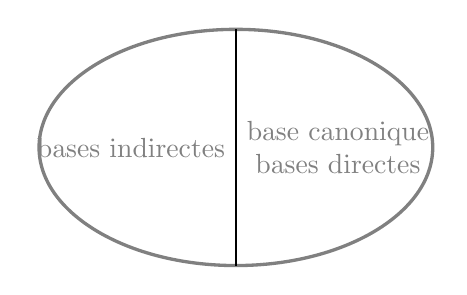
\begin{tikzpicture}
        \filldraw[color=black!50, fill=white!50, very thick] (2.5,0) ellipse (2.5 and 1.5) node[anchor=west, align=center]{base canonique\\bases directes} node[anchor=east]{bases indirectes};
        \draw[black, thick] (2.5,1.5) -- (2.5,-1.5);
    \end{tikzpicture}
\end{center}


\end{document}